%%%%%%%%%%%%%%%%%%%%%%%%%%%%%%%%%%%%%%%%%%%%%%%%%%%%%%%%%%%%%%%%%%%%%%%%%%%%%%%%
% Preámbulo                                                                    %
%%%%%%%%%%%%%%%%%%%%%%%%%%%%%%%%%%%%%%%%%%%%%%%%%%%%%%%%%%%%%%%%%%%%%%%%%%%%%%%%

\documentclass[11pt,a4paper,titlepage,oneside]{report}

%%% RELACIÓN DE VARIABLES A PERSONALIZAR %%%
\def\lingua{gal}
%\def\lingua{esp} % descomenta esta liña se redactarás a memoria en español
%\def\lingua{eng} % descomenta esta liña se redactarás a memoria en inglés
\def\nome{Mateo Amado Ares}                             % substitúe aquí o teu nome
\def\nomedirectorA{José Rouco Maseda}              % substitúe aquí o nome de quen dirixe
\def\nomedirectorB{Jorge Novo Buján}             % duplica esta liña máis veces se o precisas, cambiando
                                                     % a letra final (A, B, C, D...): úsanse na portada.tex
\def\titulo{Aliñamento de imaxes oftalmolóxicas usando representacións neuronais implícitas} % substitúe aquí o título do teu TFG
%\def\titulacion{gced}                               % descomenta esta liña e comenta a seguinte se es estudante do GCED
\def\titulacion{gei}
\def\mencion{COMPUTACIÓN}                           % descomenta a mención que che corresponda se es estudante do GEI
%\def\mencion{ENXEÑARÍA DO SOFTWARE}
%\def\mencion{ENXEÑARÍA DE COMPUTADORES}
%\def\mencion{SISTEMAS DE INFORMACIÓN}
%\def\mencion{TECNOLOXÍAS DA INFORMACIÓN}

%\def\renomearcadros{si} % descomenta esta liña se redactas a memoria en español e prefires que
                         % os "cuadros" e o "índice de cuadros" se renomeen
                         % a "tablas" e "índice de tablas" respectivamente

\usepackage{estilo_tfg}

% Lista de paquetes potencialmente interesantes (uso baixo demanda)

% \usepackage{alltt}       % proporciona o entorno alltt, semellante a verbatim pero que respecta comandos
% \usepackage{enumitem}    % permite personalizar os entornos de lista
% \usepackage{eurofont}    % proporciona o comando \euro
% \usepackage{float}       % permite máis opcións para controlar obxectos flotantes (táboas, figuras)
% \usepackage{hhline}      % permite personalizar as liñas horizontais en arrays e táboas
  \usepackage{longtable}   % permite construir táboas que ocupan máis dunha páxina
% \usepackage{lscape}      % permite colocar partes do documento en orientación apaisada
% \usepackage{moreverb}    % permite personalizar o entorno verbatim
  \usepackage{multirow}    % permite crear celdas que ocupan varias filas da mesma táboa
% \usepackage{pdfpages}    % permite insertar ficheiros en PDF no documento
% \usepackage{rotating}    % permite diferentes tipos de rotacións para figuras e táboas
% \usepackage{subcaption}  % permite a inclusión de varias subfiguras nunha figura
% \usepackage{tabu}        % permite táboas flexibles
% \usepackage{tabularx}    % permite táboas con columnas de anchura determinada

%%%%%%%%%%%%%%%%%%%%%%%%%%%%%%%%%%%%%%%%%%%%%%%%%%%%%%%%%%%%%%%%%%%%%%%%%%%%%%%%
% Corpo                                                                        %
%%%%%%%%%%%%%%%%%%%%%%%%%%%%%%%%%%%%%%%%%%%%%%%%%%%%%%%%%%%%%%%%%%%%%%%%%%%%%%%%

\begin{document}

 %%%%%%%%%%%%%%%%%%%%%%%%%%%%%%%%%%%%%%%%
 % Preliminares do documento            %
 %%%%%%%%%%%%%%%%%%%%%%%%%%%%%%%%%%%%%%%%

 \begin{titlepage}
  
  \hspace*{128pt}
  \textcolor{udcpink}{{\fontencoding{T1}\fontfamily{phv}\selectfont Facultade de Informática}}\\[-32pt]

  \begin{center}
    
\includegraphics[scale=0.3]{imaxes/udc}\\[25pt]

    {\large TRABALLO FIN DE GRAO \\
            \nometitulacion \\
            \nomemencion } \\[10pt]

    \carimbo \\[25pt]

    \begin{huge}
      \begin{spacing}{1.3}
        \bfseries \titulo
      \end{spacing}
    \end{huge}
  \end{center}
  
  \vfill
  
  \begin{flushright}
    {\large
    \begin{tabular}{ll}
      {\bf Estudante:} & \nome \\
      {\bf Dirección:} & \nomedirectorA \\
                       & \nomedirectorB \\ % duplica esta liña máis veces se o precisas, cambiando
                                           % a letra final (A, B, C, D...); define eses nomes no memoria_tfg.tex
    \end{tabular}}
  \end{flushright}
  \rightline{A Coruña, \datasimple.}
\end{titlepage}

 \dedicatoria{Dedicatoria} % escribe neste comando o teu texto de dedicatoria
 \paxinaenbranco
 \begin{agradecementos}
 \blindtext                % substitúe este comando polo teu texto de agradecementos
 \end{agradecementos}
 %%%%%%%%%%%%%%%%%%%%%%%%%%%%%%%%%%%%%%%%%%%%%%%%%%%%%%%%%%%%%%%%%%%%%%%%%%%%%%%%

\pagestyle{empty}
\begin{abstract}
O aliñamento da imaxe oftalmolóxica é un campo moi relevante. Aliñar imaxes médicas é útil para,
entre outras cousas, revisar o avance dunha enfermidade ao longo do tempo. O caso dos ollos é de particular importancia xa que permiten a observación in-vivo de tecido neuronal e vasos sanguíneos. Aliñar as imaxes manualmente é un proceso tedioso e complexo, polo que automatizar este proceso é moi beneficioso.

Neste traballo explórase o uso de redes de representación implícita,
 onde se parametriza a imaxe como unha función continua coas coordenadas como entrada e o valor do pixel como saída, como unha alternativa para o aliñamento de imaxes.
 Estas aportan vantaxes frente a representacións tradicionais discretas como a independencia de resolución e poder prescindir de grandes bases de datos xa que se adestran mediante un proceso de optimización para cada par de imaxes.
 Ademais, en lugar de usar funcións de activación estándar como RELU, adoitan empregar unha función de activación sinusoidal (SIREN), que pode axudar a eliminar o sesgo cara sinais de baixa frecuencia e mapear mellor deformación pequenas e detalladas.

Adaptando o traballo realizado por \cite{wolterink2021implicit}, valoraráse se este método é apto para a tarefa de aliñamento de imaxes oftalmolóxicas e como se compara con métodos convencionais.

  \vspace*{25pt}
  \begin{segundoresumo}
    Ophthalmic image alignment is a highly relevant field. Aligning medical images is useful for, among other things, reviewing the progression of a disease over time. The case of eyes is particularly important as they allow in-vivo observation of neuronal tissue and blood vessels. Manually aligning images is a tedious and complex process, so automating this process is beneficial.
    
    This work explores the use of implicit representation networks, where the image is parameterized as a continuous function with coordinates as input and pixel value as output. This provides advantages over traditional discrete representations such as resolution independence and the ability to dispense with large databases since they are trained through an optimization process for each group of images.
    Furthermore, instead of using standard activation functions like RELU, they typically employ a sinusoidal activation function (SIREN), which can help eliminate bias towards low-frequency signals and better map small and detailed deformations.
    
    Based on the work done by \cite{wolterink2021implicit}, this study will evaluate whether this method is suitable for the task of aligning ophthalmic images and how it compares to conventional methods.
  \end{segundoresumo}
\vspace*{25pt}
\begin{multicols}{2}
  \begin{description}
  \item [\palabraschaveprincipal:] \mbox{} \\[-20pt]
  \begin{itemize}
      \item Imagen médica
      \item Imagen oftalmológica
      \item Aprendizaje profundo
      \item Registro de Imágenes 
      \item Representaciones neuronales implícitas
  \end{itemize}
  
  \end{description}
  \begin{description}
  \item [\palabraschavesecundaria:] \mbox{} \\[-20pt]
  \begin{itemize}
      \item Medical imaging
      \item Ophthalmological imaging
      \item Deep learning
      \item Image Registration
      \item Implicit neural representations (INRs)
  \end{itemize}
  \end{description}
  \end{multicols}
\end{abstract}
\pagestyle{fancy}

%%%%%%%%%%%%%%%%%%%%%%%%%%%%%%%%%%%%%%%%%%%%%%%%%%%%%%%%%%%%%%%%%%%%%%%%%%%%%%%%


 \pagenumbering{roman}
 \setcounter{page}{1}
 \bstctlcite{IEEEexample:BSTcontrol}

 \tableofcontents
 \listoffigures
 \listoftables
 \clearpage
 
 \pagenumbering{arabic}
 \setcounter{page}{1}

 %%%%%%%%%%%%%%%%%%%%%%%%%%%%%%%%%%%%%%%%
 % Capítulos                            %
 %%%%%%%%%%%%%%%%%%%%%%%%%%%%%%%%%%%%%%%%

 \chapter{Introdución}
\label{chap:introducion}

\lettrine{P}{rimer} capítulo da memoria, onde xeralmente se exporán as
liñas mestras do traballo, os obxectivos, etc. Incluimos un par de
exemplos de citas~\cite{ErlangBook,ErlangWebBook} e de referencias
internas (sección \ref{sec:mostra}, páxina \pageref{sec:mostra}).

\Blindtext

\section{Sección de mostra}
\label{sec:mostra}

\Blindtext

\subsection{Subsección de mostra}

\Blindtext

 \chapter{Contido demostrativo}
\label{chap:demo}

\lettrine{E}{ntre} a introdución e as conclusións, o documento conterá
tantos capítulos como sexa preciso, sempre con coidado de non rebasar
o límite de 80 páxinas fixado polo regulamento de TFGs.

Empregaremos éste de xeito demostrativo, para ilustrar o uso de
elementos habituais que poidan ser de utilidade\footnote{Por exemplo,
  isto é unha nota a pé de páxina.}.

\section{Inclusión de imaxes}

Se precisamos imaxes no noso documento, incluirémolas do xeito que se
indica na figura~\ref{fig:exemplo} (páxina~\pageref{fig:exemplo}). Se
o facemos así, \LaTeX ubicará cada imaxe no mellor lugar posible,
lugar que pode variar a medida que o documento vaia crecendo coa
inclusión de máis texto e outros elementos (máis imaxes, táboas,
etc.).

\begin{figure}[hp!]
  \centering
  
\includegraphics[width=0.75\textwidth]{imaxes/udc.png}
  \caption{Pé de imaxe descritivo}
  \label{fig:exemplo}
\end{figure}

Recoméndase almacenar os ficheiros gráficos no directorio
\texttt{imaxes}.

\subsection{Inclusión de varias sub-imaxes}

Se precisamos inserir imaxes relacionadas, pode ser apropiado
incluílas como sub-figuras, do xeito que se pode apreciar na
figura~\ref{fig:exemplo-subfiguras} (páxina~\pageref{fig:exemplo-subfiguras})
coas imaxes~\ref{fig:subfigura-rotada} e~\ref{fig:subfigura-deformada}.
Como se pode ver nos exemplos desta sección, sempre é recomendable
referirse ás imaxes (ou táboas e outros elementos \emph{flotantes},
que se demostrarán nas seccións seguintes deste capítulo demostrativo)
pola súa referencia, xa que dese xeito non dependemos de onde
queden ubicados os elementos en cuestión.

\begin{figure}[hp!]
  \centering
  \begin{subfigure}[c]{0.3\textwidth}
    
\includegraphics[angle=45,width=\textwidth]{imaxes/udc.png}
    \caption{Pé de subimaxe rotada}
    \label{fig:subfigura-rotada}
  \end{subfigure}
  \hspace{0.1\textwidth}
  \begin{subfigure}[c]{0.3\textwidth}
    
\includegraphics[width=\textwidth,height=3cm]{imaxes/udc.png}
    \caption{Pé de subimaxe deformada}
    \label{fig:subfigura-deformada}
  \end{subfigure}
  \caption{Pé de imaxe xeral}
  \label{fig:exemplo-subfiguras}
\end{figure}

\section{Inclusión de táboas}

Se precisamos táboas no noso documento, incluirémolas do xeito que se
indica na táboa~\ref{tab:exemplo} (páxina~\pageref{tab:exemplo}). Se
o facemos así, \LaTeX ubicará cada táboa no mellor lugar posible,
lugar que pode variar a medida que o documento vaia crecendo coa
inclusión de máis texto e outros elementos (máis imaxes, táboas,
etc.).

\begin{table}[hp!]
  \centering
  \rowcolors{2}{white}{udcgray!25}
  \begin{tabular}{c|c}
  \rowcolor{udcpink!25}
  \textbf{Título de columna} & \textbf{Outro título de columna} \\\hline
  \textit{Título de fila} & Contido da cela \\
  \textit{Título de fila} & Contido da cela \\
  \textit{Título de fila} & Contido da cela \\
  \textit{Título de fila} & Contido da cela \\
  \textit{Título de fila} & Contido da cela \\
  \textit{Título de fila} & Contido da cela \\
  \end{tabular}
  \caption{Pé de táboa descritivo}
  \label{tab:exemplo}
\end{table}

\subsection{Inclusión de táboas longas}

Para táboas longas que ocupan varias páxinas, como é o caso da \ref{tab:longa}
(páxina~\pageref{tab:longa}), recoméndase o uso do paquete \texttt{lontable},
incluído xa entre os paquetes recomendados no ficheiro raíz do proxecto
(\verb+memoria_tfg.tex+).

{\rowcolors{2}{white}{udcgray!25}
\begin{longtable}{l|r|c}
  \caption{Pé descritivo dunha táboa longa}
  \label{tab:longa} \\

  \rowcolor{udcpink!25}
  \textbf{Primeira columna} & \textbf{Segunda columna} & \textbf{Terceira columna} \\\hline
  \endfirsthead

  \multicolumn{3}{c}{\tablename\ \thetable{} -- {\small \textit{(vén da páxina anterior)}}} \\
  \rowcolor{udcpink!25}
  \textbf{Primeira columna} & \textbf{Segunda columna} & \textbf{Terceira columna} \\\hline
  \endhead

  \multicolumn{3}{c}{\dotfill{\small \textit{(continúa na páxina seguinte)}}\dotfill} \\
  \endfoot

  \endlastfoot

  Texto de exemplo & abcdef ghjijklmn & 123.456778 \\
  Texto de exemplo & abcdef ghjijklmn & 123.456778 \\
  Texto de exemplo & abcdef ghjijklmn & 123.456778 \\
  Texto de exemplo & abcdef ghjijklmn & 123.456778 \\
  Texto de exemplo & abcdef ghjijklmn & 123.456778 \\
  Texto de exemplo & abcdef ghjijklmn & 123.456778 \\
  Texto de exemplo & abcdef ghjijklmn & 123.456778 \\
  Texto de exemplo & abcdef ghjijklmn & 123.456778 \\
  Texto de exemplo & abcdef ghjijklmn & 123.456778 \\
  Texto de exemplo & abcdef ghjijklmn & 123.456778 \\
  Texto de exemplo & abcdef ghjijklmn & 123.456778 \\
  Texto de exemplo & abcdef ghjijklmn & 123.456778 \\
  Texto de exemplo & abcdef ghjijklmn & 123.456778 \\
  Texto de exemplo & abcdef ghjijklmn & 123.456778 \\
  Texto de exemplo & abcdef ghjijklmn & 123.456778 \\
  Texto de exemplo & abcdef ghjijklmn & 123.456778 \\
  Texto de exemplo & abcdef ghjijklmn & 123.456778 \\
  Texto de exemplo & abcdef ghjijklmn & 123.456778 \\
  Texto de exemplo & abcdef ghjijklmn & 123.456778 \\
  Texto de exemplo & abcdef ghjijklmn & 123.456778 \\
  Texto de exemplo & abcdef ghjijklmn & 123.456778 \\
  Texto de exemplo & abcdef ghjijklmn & 123.456778 \\
  Texto de exemplo & abcdef ghjijklmn & 123.456778 \\
  Texto de exemplo & abcdef ghjijklmn & 123.456778 \\
  Texto de exemplo & abcdef ghjijklmn & 123.456778 \\
  Texto de exemplo & abcdef ghjijklmn & 123.456778 \\
  Texto de exemplo & abcdef ghjijklmn & 123.456778 \\
  Texto de exemplo & abcdef ghjijklmn & 123.456778 \\
  Texto de exemplo & abcdef ghjijklmn & 123.456778 \\
  Texto de exemplo & abcdef ghjijklmn & 123.456778 \\
  Texto de exemplo & abcdef ghjijklmn & 123.456778 \\
  Texto de exemplo & abcdef ghjijklmn & 123.456778 \\
  Texto de exemplo & abcdef ghjijklmn & 123.456778 \\
  Texto de exemplo & abcdef ghjijklmn & 123.456778 \\
  Texto de exemplo & abcdef ghjijklmn & 123.456778 \\
  Texto de exemplo & abcdef ghjijklmn & 123.456778 \\
  Texto de exemplo & abcdef ghjijklmn & 123.456778 \\

\end{longtable}
} % alcance do rowcolors que precede á táboa longa


\subsection{Inclusión de táboas con celas que ocupan varias columnas ou filas}

En ocasións pode resultar de interese incluír nunha táboa unha cela que se estenda
a través de varias columnas, como ocorre na táboa~\ref{tab:exemplocolumnas}
(páxina~\pageref{tab:exemplocolumnas}).

\begin{table}[hp!]
  \centering
  \rowcolors{2}{white}{udcgray!25}
  \begin{tabular}{c|c|c}
  \rowcolor{udcpink!25}
  \multicolumn{3}{c}{\textbf{Cela en varias columnas}} \\\hline
  \rowcolor{udcpink!25}
  \textbf{Título de columna} & \textbf{Outro título de columna} & \textbf{Outro título máis} \\\hline
  \textit{Título de fila}    & Contido da cela                  & Contido da cela \\
  \textit{Título de fila}    & Contido da cela                  & Contido da cela \\
  \textit{Título de fila}    & \multicolumn{2}{c}{Contido da cela múltiple} \\
  \textit{Título de fila}    & Contido da cela                  & Contido da cela \\
  \end{tabular}
  \caption{Pé de táboa descritivo (táboa con celas que ocupan varias columnas)}
  \label{tab:exemplocolumnas}
\end{table}

Tamén pode resultar necesario facer o propio mais en varias filas da mesma columna,
como ocorre na táboa~\ref{tab:exemplofilas} (páxina~\pageref{tab:exemplofilas}).
Para isto é preciso o paquete \texttt{multirow}, incluído entre os recomendados no
ficheiro raíz do proxecto (\verb+memoria_tfg.tex+).

O uso de celas multifila requerirá do xuste da coloración das filas, a fin de manter
a coherencia entre o contido e o continente. Así, no canto de usar un único comando
\verb+rowcolors+ para indicar a alternancia en toda a táboa, usaremos o comando
\verb+rowcolor+ antes dunha fila que queiramos colorear, e o comando \verb+cellcolor+
dentro dunha cela que queiramos colorear.

\begin{table}[hp!]
  \centering
  \begin{tabular}{c|c}
  \rowcolor{udcpink!25}
  \textbf{Título de columna} & \textbf{Outro título de columna} \\\hline
  \multirow{2}{*}{\textit{Título de fila}} & \cellcolor{udcgray!25} Contido da cela \\
                                           & Contido da cela \\
  \rowcolor{udcgray!25}
  \textit{Título de fila}                  & Contido da cela \\
  \multirow{3}{*}{\textit{Título de fila}} & Contido da cela \\
                                           & \cellcolor{udcgray!25} Contido da cela \\
                                           & Contido da cela \\
  \rowcolor{udcgray!25}
  \textit{Título de fila}                  & Contido da cela \\
  \end{tabular}
  \caption{Pé de táboa descritivo (táboa con celas que ocupan varias filas)}
  \label{tab:exemplofilas}
\end{table}

Por suposto, pódense combinar nunha mesma táboa os dous tipos de celas (as que se 
estenden máis dunha fila e máis dunha columna), como na táboa~\ref{tab:exemplofilasecolumnas}
(páxina~\pageref{tab:exemplofilasecolumnas}).

\begin{table}[hp!]
  \centering
  \begin{tabular}{c|c|c}
  \rowcolor{udcpink!25}
  \multicolumn{3}{c}{\textbf{Cela en varias columnas}} \\\hline
  \rowcolor{udcpink!25}
  \textbf{Título de columna}               & \textbf{Outro título de columna}             & \textbf{Outro título máis} \\\hline
  \multirow{2}{*}{\textit{Título de fila}} & \cellcolor{udcgray!25} Contido da cela       & \cellcolor{udcgray!25} Contido da cela \\
                                           & Contido da cela                              & Contido da cela \\
  \rowcolor{udcgray!25}
  \textit{Título de fila}                  & \multicolumn{2}{c}{Contido da cela múltiple} \\
  \multirow{3}{*}{\textit{Título de fila}} & Contido da cela                              & Contido da cela \\
                                           & \multicolumn{2}{c}{\cellcolor{udcgray!25} Contido da cela múltiple} \\
                                           & \multicolumn{2}{c}{Contido da cela múltiple} \\
  \rowcolor{udcgray!25}
  \textit{Título de fila}                  & Contido da cela                              & Contido da cela \\
  \end{tabular}
  \caption{Pé de táboa descritivo (táboa con celas que ocupan varias columnas)}
  \label{tab:exemplofilasecolumnas}
\end{table}

\section{Inclusión de código fonte}

Se precisamos incluír fragmentos de código fonte, podemos facelo, por exemplo, da
seguinte maneira:

\begin{lstlisting}[language=C]
#include <stdio.h>
#define N 10

int main()
{
  int i;

  // Isto é un comentario
  puts("Ola, mundo!");

  for (i = 0; i < N; i++)
  {
    puts("LaTeX é a ferramenta de edición ideal para profesionais da informática!");
  }

  return 0;
}
\end{lstlisting}

\section{Uso da relación de acrónimos e do glosario}

Os acrónimos edítanse no ficheiro \texttt{bibliografia/acronimos.tex}
e úsanse empregando a orde \texttt{acrlong} para obter o termo
completo (deste xeito: \acrlong{erlang}), a orde \texttt{acrshort}
para obter o acrónimo (deste xeito: \acrshort{erlang}). A primeira vez
que usamos un termo con acrónimo no documento é recomendable usar orde
\texttt{acrfull} (que produce ambas versións á vez:
\acrfull{erlang}). Os acrónimos que non se usan no documento, non
aparecen na relación que se xerar na versión PDF.

Pola súa banda, os termos do glosario edítanse no ficheiro
\texttt{bibliografia/glo\-sa\-rio.tex} e úsanse empregando a orde
\texttt{gls} (deste xeito, \gls{bytecode}) ou \texttt{Gls} (deste
xeito, \Gls{bytecode}). Ao igual que os acrónimos, os termos que non
se usan no documento, non aparecen na relación que se xera na versión
PDF.

%\include{contido/...}
 \chapter{Conclusións}
\label{chap:conclusions}

\lettrine{D}{erradeiro} capítulo da memoria, onde se presentará a
situación final do traballo, as leccións aprendidas, a relación coas
competencias da titulación en xeral e a mención en particular,
posibles liñas futuras,\dots

\Blindtext


 %%%%%%%%%%%%%%%%%%%%%%%%%%%%%%%%%%%%%%%%
 % Apéndices, glosarios e bibliografía  %
 %%%%%%%%%%%%%%%%%%%%%%%%%%%%%%%%%%%%%%%%

 \appendix
 \appendixpage
 \chapter{Material adicional}
\label{chap:adicional}

\section{Anexo regularization}
\label{sec:Anexo regularization}

% \begin{table}[h]
%     \centering
%     \begin{minipage}[t]{0.45\linewidth}
%         \centering
%         \scriptsize
%         \setlength{\tabcolsep}{25pt}
%         \begin{tabular}{|c|c|}
%         \hline
%         Resolution & Mean Distance \\ \hline
%         100 & 254.22 \\ \hline
%         250 & 251.29 \\ \hline
%         750 & 250.62 \\ \hline
%         1250 & 250.59 \\ \hline
%         1708 & 249.72 \\ \hline
%         \end{tabular}
%         \caption{Distancias medias para o dataset FIRE ca función de activación Relu}
%         \label{tab:mlp_mean_distances_fire}
%     \end{minipage}
%     \hfill
%     \begin{minipage}[t]{0.45\linewidth}
%         \centering
%         \scriptsize
%         \setlength{\tabcolsep}{25pt}
%         \begin{tabular}{|c|c|}
%         \hline
%         Resolution & Mean Distance \\ \hline
%         100 & 266.43 \\ \hline
%         250 & 263.85 \\ \hline
%         750 & 263.19 \\ \hline
%         1250 & 258.56 \\ \hline
%         1708 & 258.06 \\ \hline
%         \end{tabular}
%         \caption{Distancias medias para o dataset FIRE ca función de activación SIREN}
%         \label{tab:siren_mean_distances_fire}
%     \end{minipage}
% \end{table}

% \begin{table}[h]
%     \centering
%     \begin{minipage}[t]{0.45\linewidth}
%         \centering
%         \scriptsize
%         \setlength{\tabcolsep}{25pt}
%         \begin{tabular}{|c|c|}
%         \hline
%         Resolution & Mean Distance \\ \hline
%         100 & 37.29 \\ \hline
%         250 & 36.18 \\ \hline
%         750 & 36.01 \\ \hline
%         1250 & 35.03 \\ \hline
%         1708 & 35.04 \\ \hline
%         \end{tabular}
%         \caption{Distancias medias para o dataset RFMID ca función de activación Relu}
%         \label{tab:mlp_mean_distances_rfmid}
%     \end{minipage}
%     \hfill
%     \begin{minipage}[t]{0.45\linewidth}
%         \centering
%         \scriptsize
%         \setlength{\tabcolsep}{25pt}
%         \begin{tabular}{|c|c|}
%         \hline
%         Resolution & Mean Distance \\ \hline
%         100 & 68.12 \\ \hline
%         250 & 73.42 \\ \hline
%         750 & 77.55 \\ \hline
%         1250 & 67.33 \\ \hline
%         1708 & 67.31 \\ \hline
%         \end{tabular}
%         \caption{Distancias medias para o dataset RMIFD ca función de activación SIREN}
%         \label{tab:siren_mean_distances_rfmid}
%     \end{minipage}
% \end{table}


\subsection{Figuras experimentos de regularización}
\label{subsec:figuras_experimentos_regularizacion}

\paragraph{Resultados}
\label{par:Resultados-reg2}

Os resultados da experimentación extendida da regularización, realizados sobre os datasets FIRE e RFMID, preséntanse nas figuras \ref{fig:gs_single_heatmaps}.

\begin{figure}[tbp]
    \centering
    \begin{subfigure}[b]{0.4\textwidth}
        \centering
        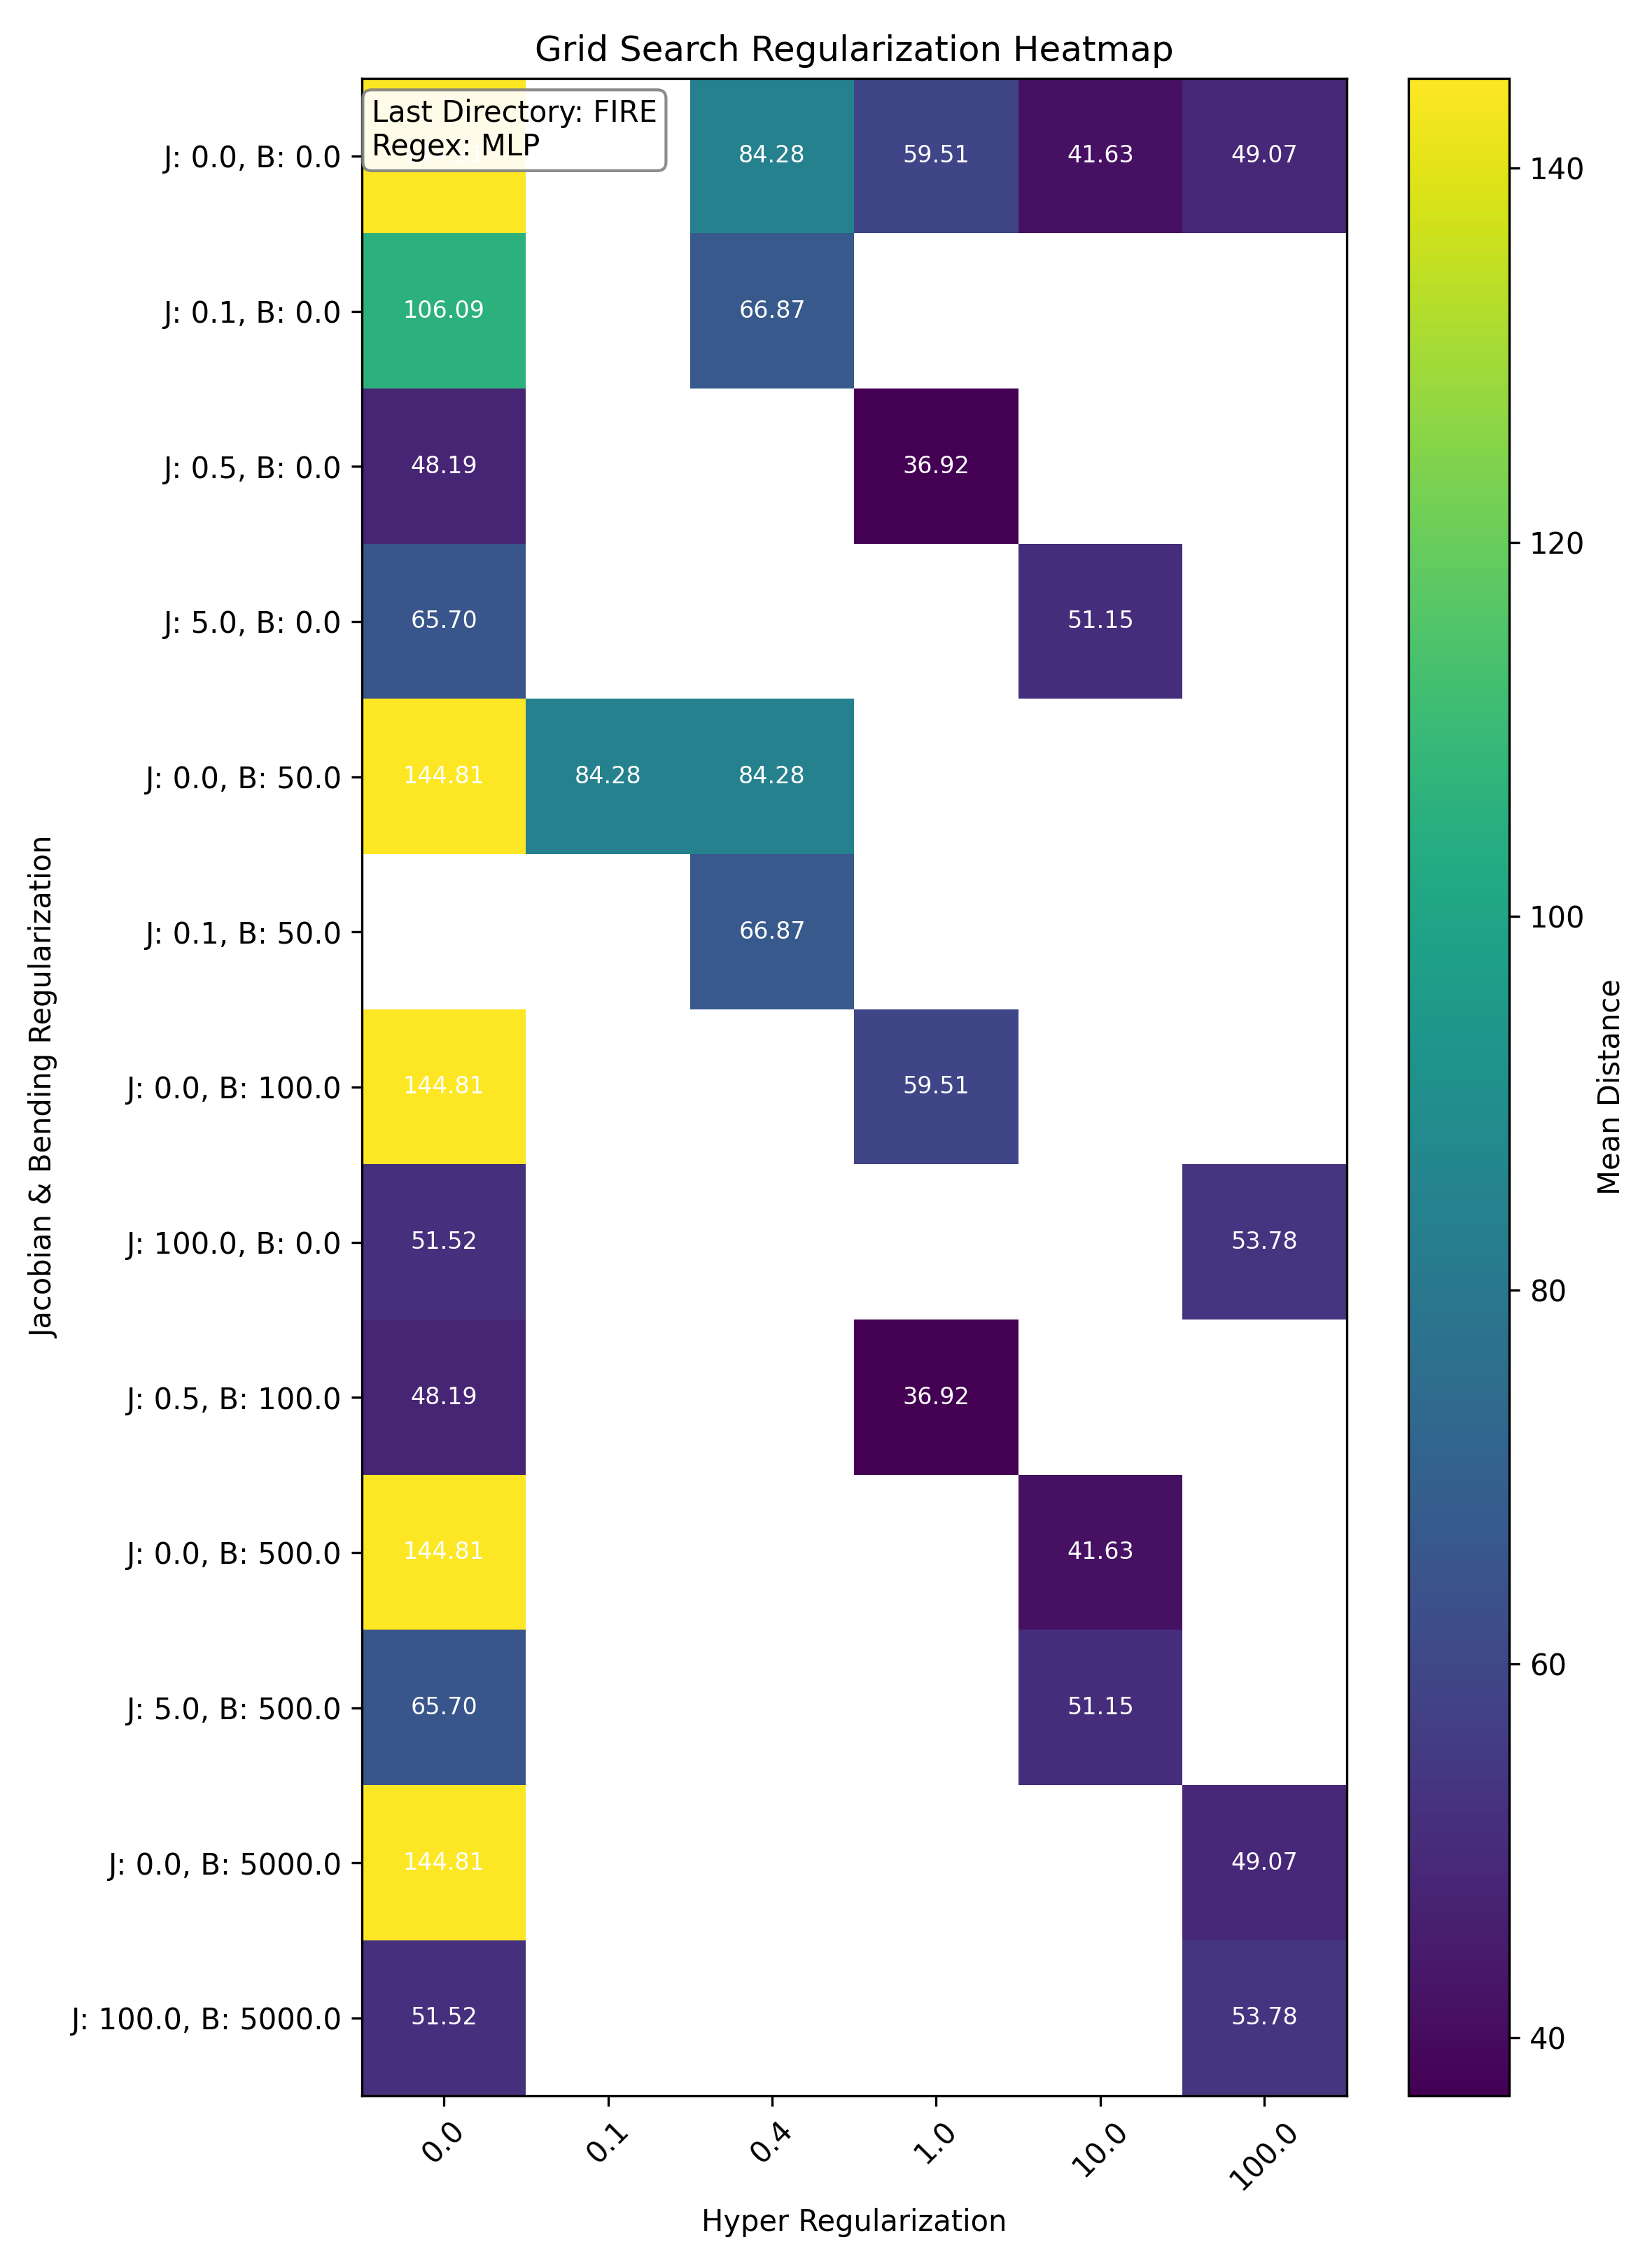
\includegraphics[width=\textwidth]{imaxes/grid_search_single_heatmap_FIRE_MLP.png}
        \caption{FIRE - Relu}
        \label{fig:gs_single_FIRE_MLP}
    \end{subfigure}\hfill
    \begin{subfigure}[b]{0.4\textwidth}
        \centering
        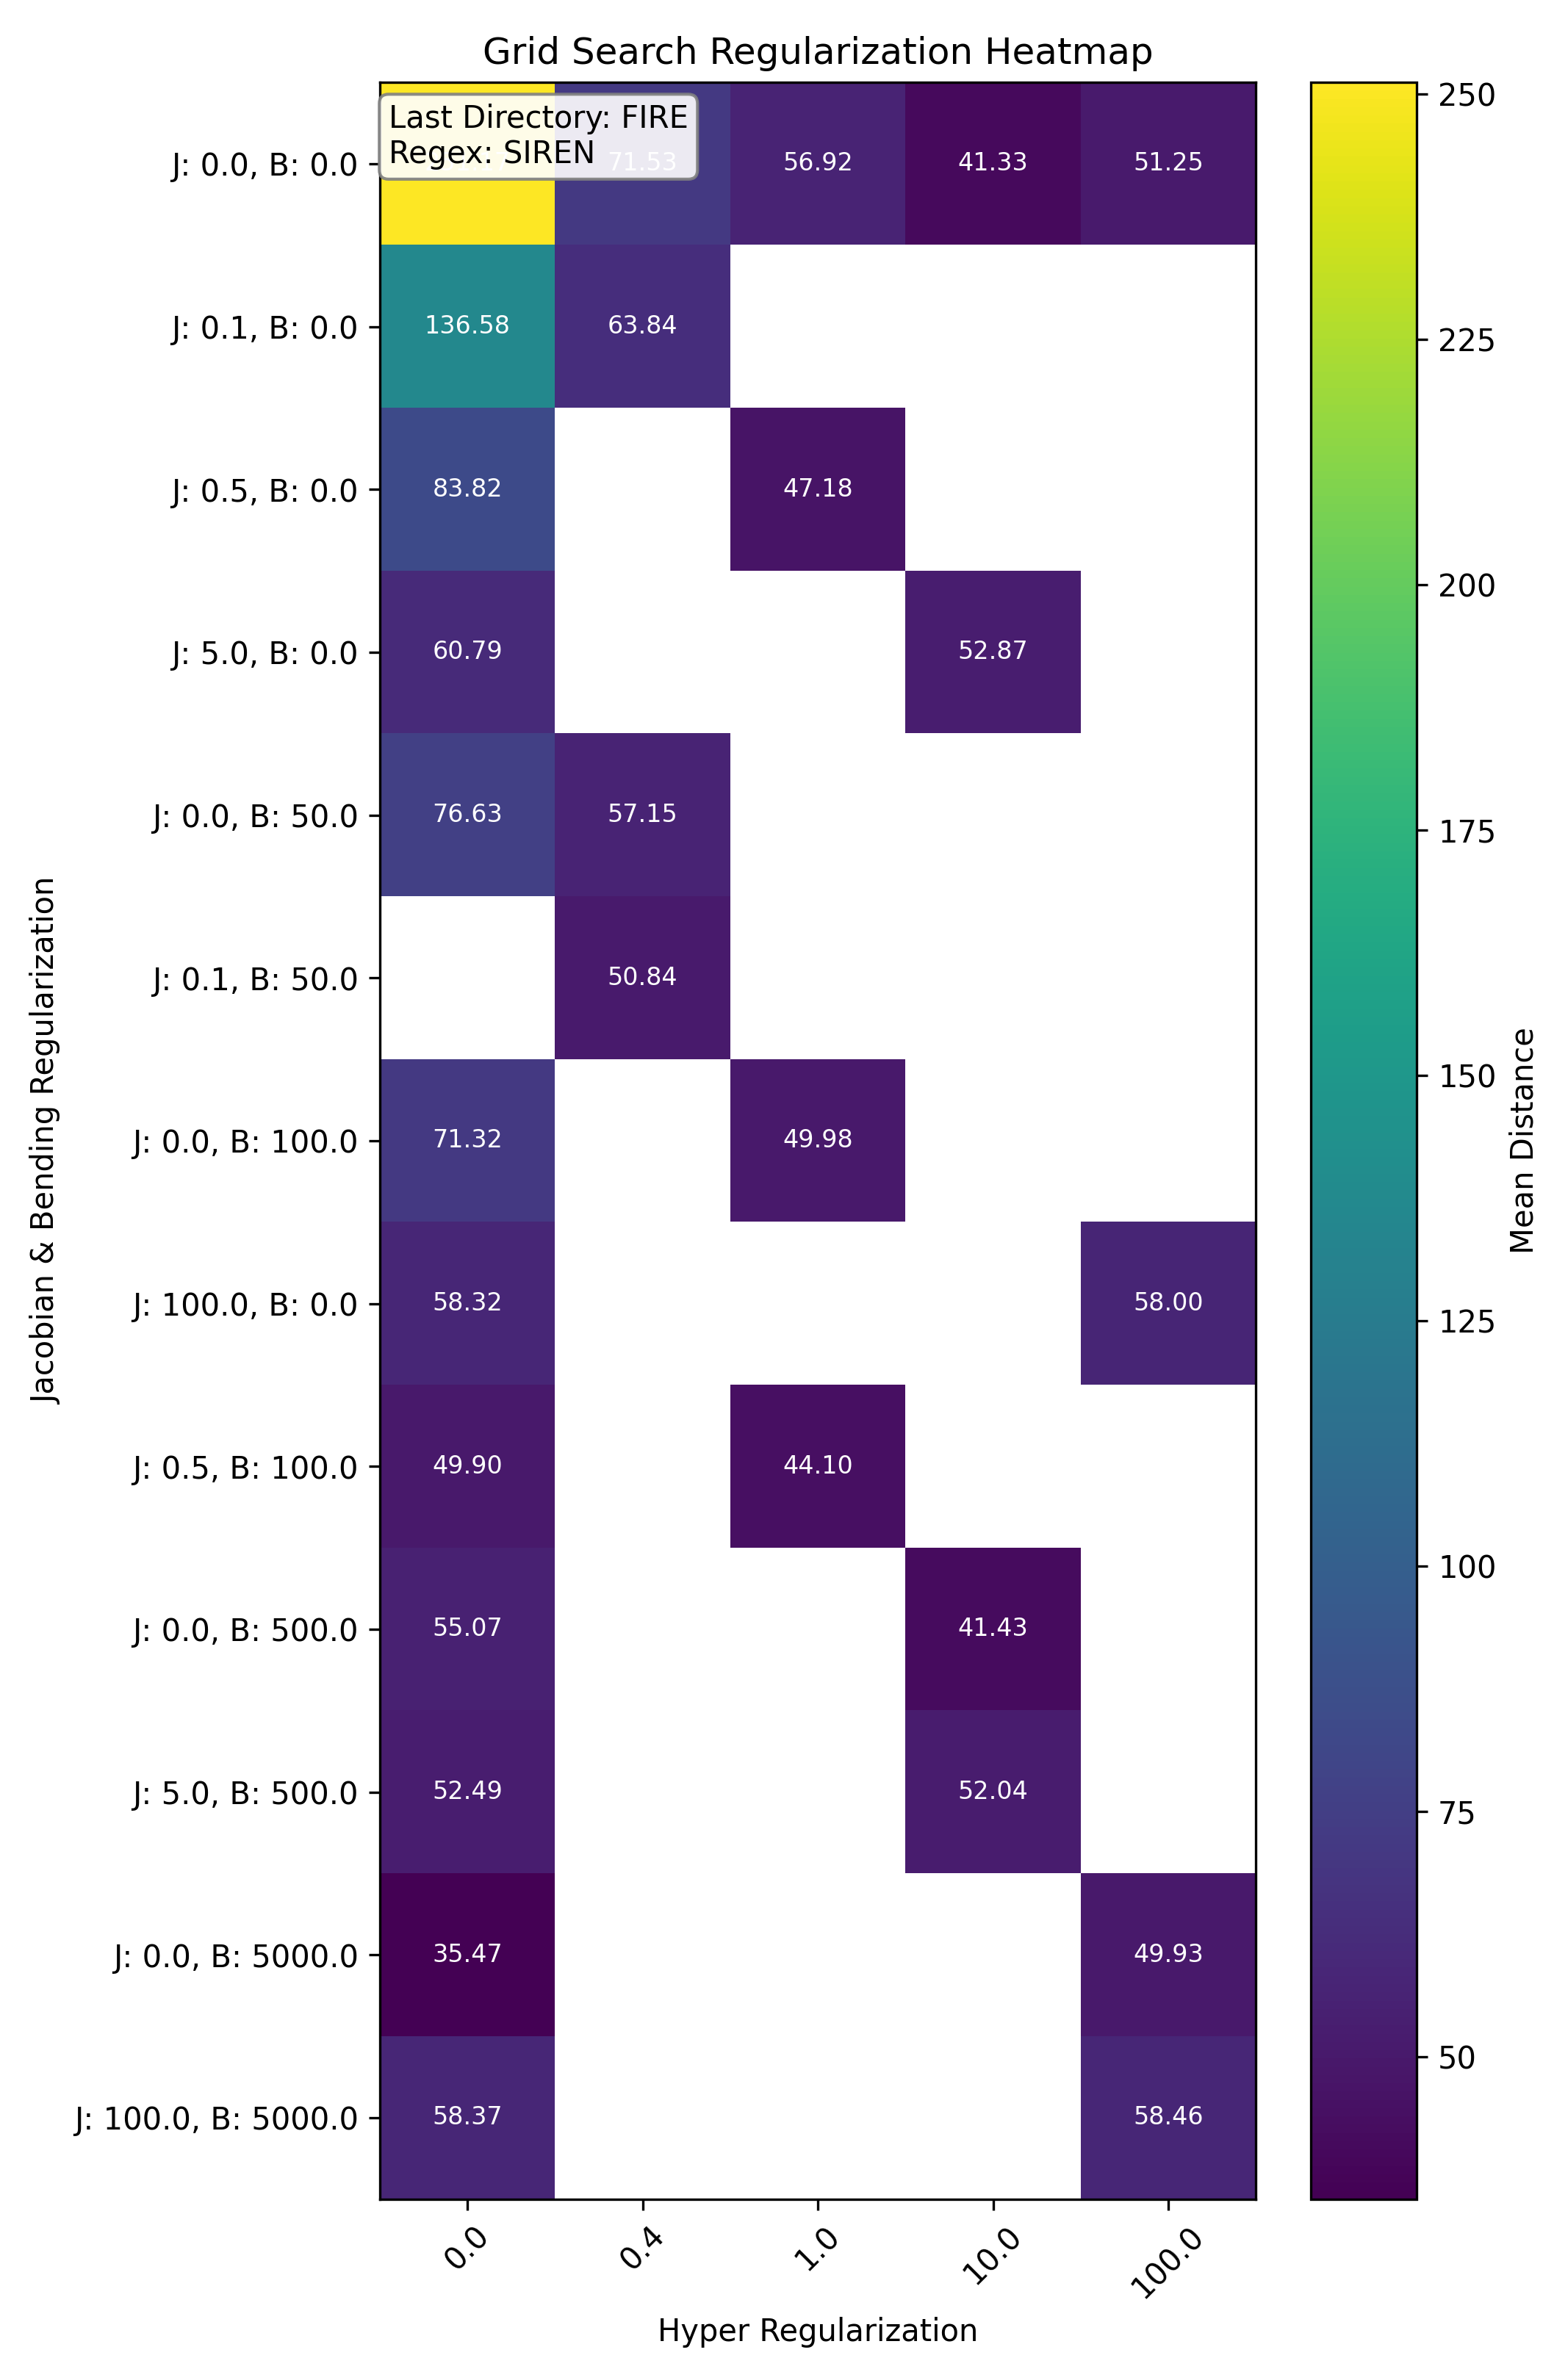
\includegraphics[width=\textwidth]{imaxes/grid_search_single_heatmap_FIRE_SIREN.png}
        \caption{FIRE - SIREN}
        \label{fig:gs_single_FIRE_SIREN}
    \end{subfigure}
    
    \vskip0\baselineskip
    
    \begin{subfigure}[b]{0.4\textwidth}
        \centering
        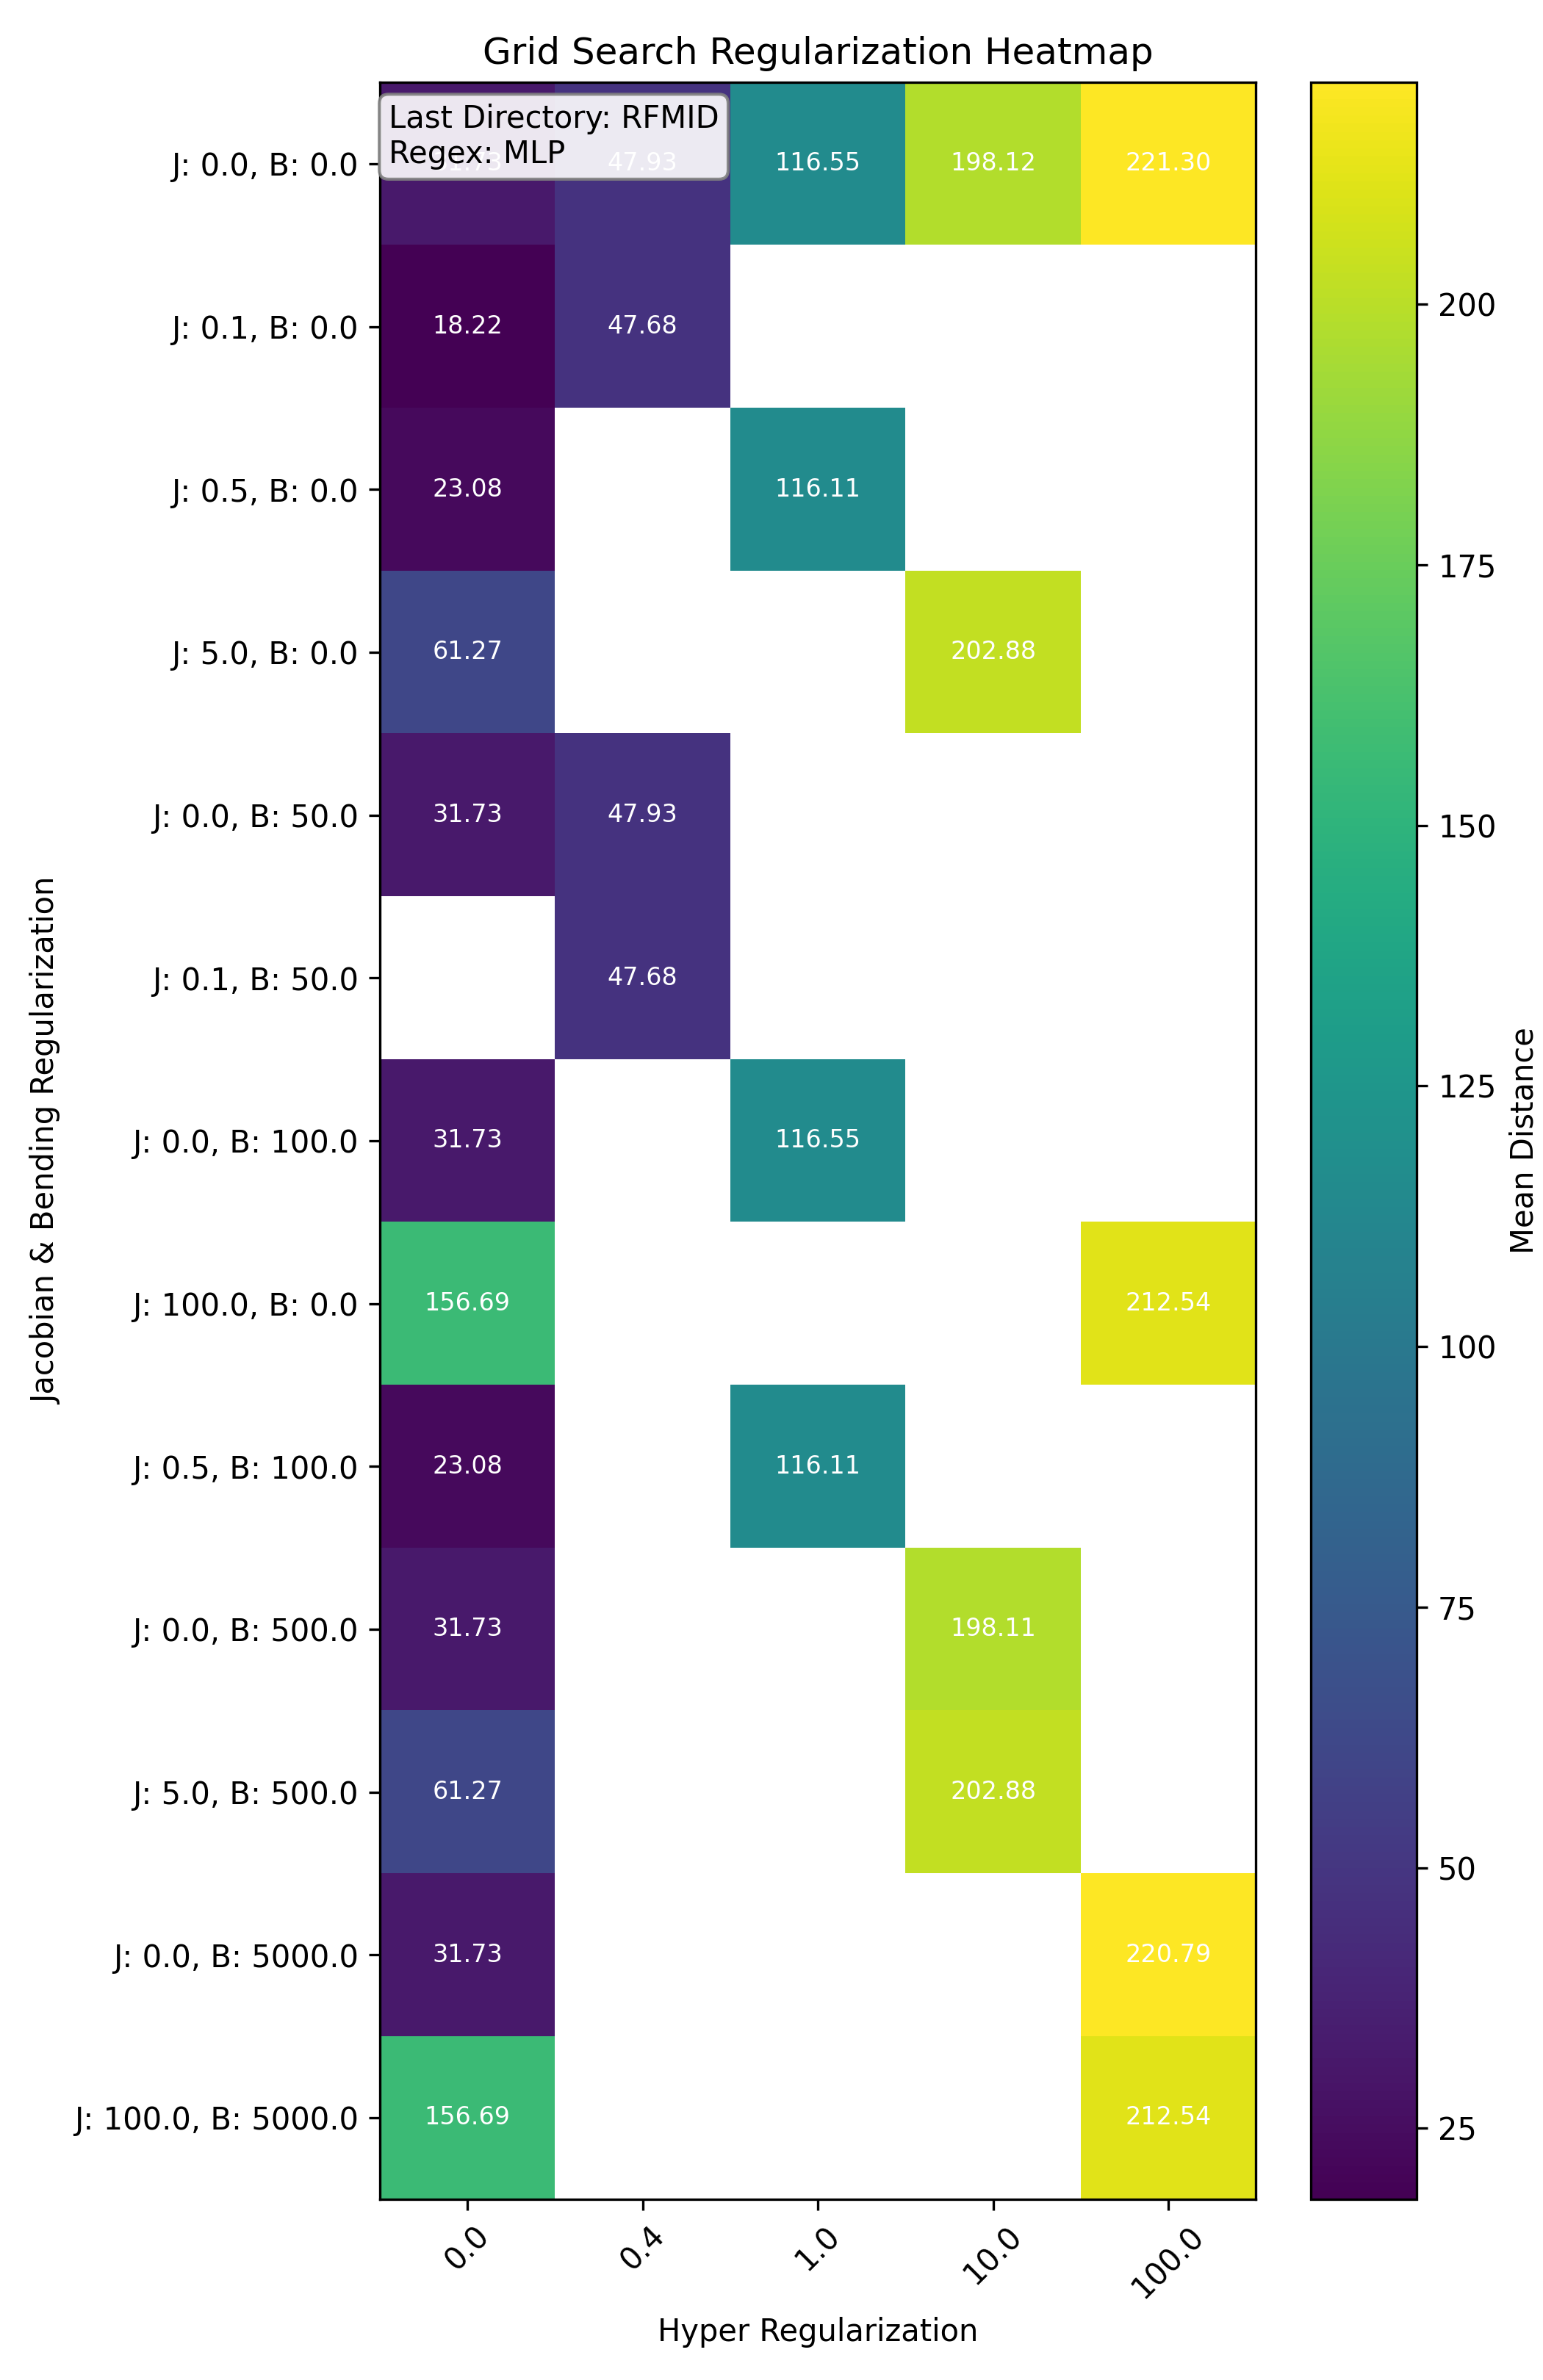
\includegraphics[width=\textwidth]{imaxes/grid_search_single_heatmap_RFMID_MLP.png}
        \caption{RFMID - Relu}
        \label{fig:gs_single_RFMID_MLP}
    \end{subfigure}\hfill
    \begin{subfigure}[b]{0.4\textwidth}
        \centering
        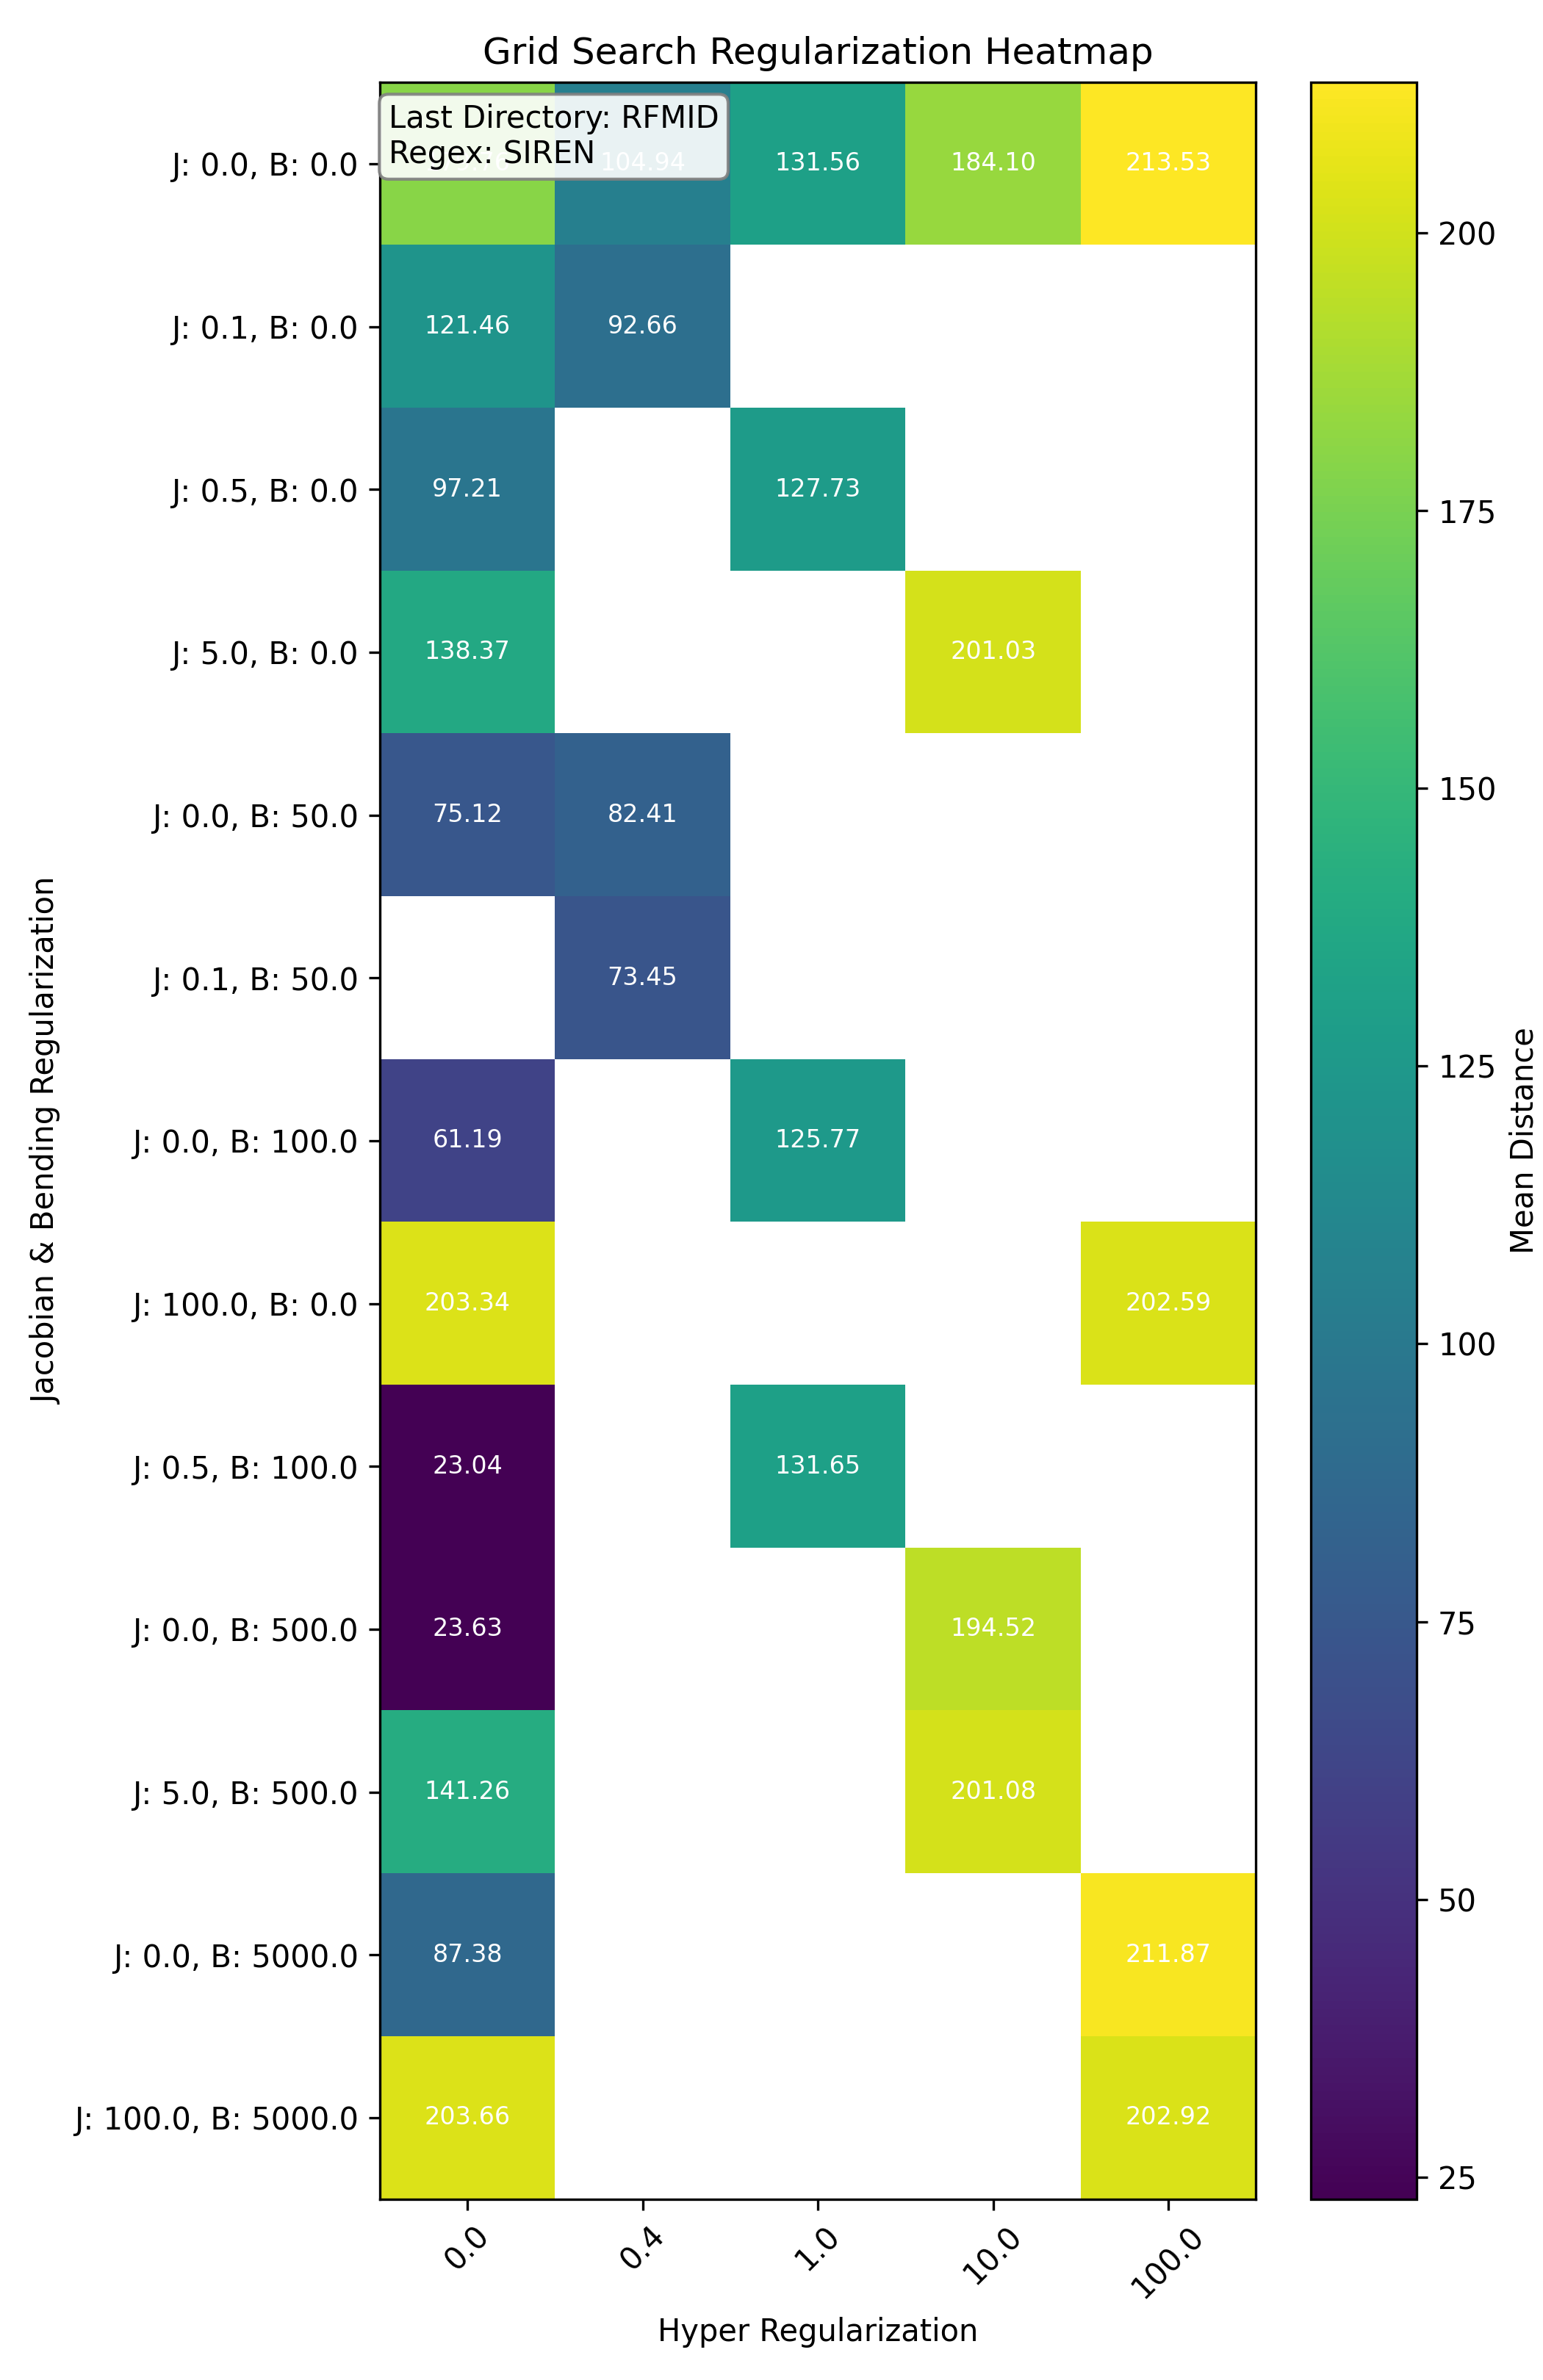
\includegraphics[width=\textwidth]{imaxes/grid_search_single_heatmap_RFMID_SIREN.png}
        \caption{RFMID - SIREN}
        \label{fig:gs_single_RFMID_SIREN}
    \end{subfigure}
    
    \caption{Mapa de calor cos resultados de diferentes combinacións de termos de regularización e funcións de activación sobre os datasets FIRE e RFMID}
    \label{fig:gs_single_heatmaps}
\end{figure}

\paragraph{Discusión}
\label{par:Discusion-reg2}

Os resultados amosan que as interaccións entre os diferentes termos de regularización e as funcións de activación son complexas e moi dependentes da parella de imaxes concreta a rexistrar.

\FloatBarrier
%\include{anexos/...}

 \printglossary[type=\acronymtype,title=\nomeglosarioacronimos]
 \printglossary[title=\nomeglosariotermos]

 \bibliographystyle{IEEEtranN}
 \bibliography{\bibconfig,bibliografia/bibliografia}
 \clearpage
 
\end{document}

%%%%%%%%%%%%%%%%%%%%%%%%%%%%%%%%%%%%%%%%%%%%%%%%%%%%%%%%%%%%%%%%%%%%%%%%%%%%%%%%
